\section{Results}

% Main numeric anchors:
% - tables/model_validation_table.csv
% - tables/grid_size_summary_table.csv
% - tables/district_benchmark_metrics_table.csv
% - tables/external_benchmark_summary_table.csv
% - tables/ablation_summary_table.csv
% - tables/qualitative_validation_case_table.csv
% - source_text/paper_report_summary.md

\subsection{Model choice}

In the frozen baseline, the random forest model outperformed the ridge comparator. Under leave-one-city-out validation, random forest achieved a calibrated RMSE of 115.934 and a calibrated $R^2$ of 0.934. The strongest validation row overall also came from random forest under spatial block cross-validation, with a calibrated RMSE of 76.301, but the production identity of v2 remains centered on the random forest model, the 500\,m grid, and calibrated-only output.

This model split is substantively useful rather than merely procedural. The contrast between random forest and ridge is consistent with a proxy-population problem in which the relationship between urban structure and population concentration is unlikely to be globally linear. Built form, floor area, transport structure, and service-access signals can interact in ways that are difficult to capture through a single linear weighting surface, especially once the target itself is constructed through weak supervision. Within the frozen v2 evidence stack, the stronger performance of random forest therefore supports the choice of a flexible non-linear baseline without implying that the model recovers cell-level truth.

\subsection{Grid choice}

The grid-size benchmark supported 500\,m as the frozen default. This configuration achieved the best benchmark score (0.248572) among the three tested options and provides a practical balance between spatial detail and surface stability.

This result is also interpretable in operational terms. The 250\,m configuration provides finer nominal detail, but it also creates many more cells and increases the risk that sparse feature support or local fragmentation will dominate the signal. At the other extreme, the 1000\,m configuration is operationally simpler but more likely to smooth away meaningful intra-urban variation that the baseline is intended to preserve. The 500\,m grid is therefore justified not only by its benchmark score but also by its practical role as a middle ground between excessive fragmentation and excessive smoothing.

\begin{figure}[H]
\centering
\begin{subfigure}[t]{0.48\textwidth}
    \centering
    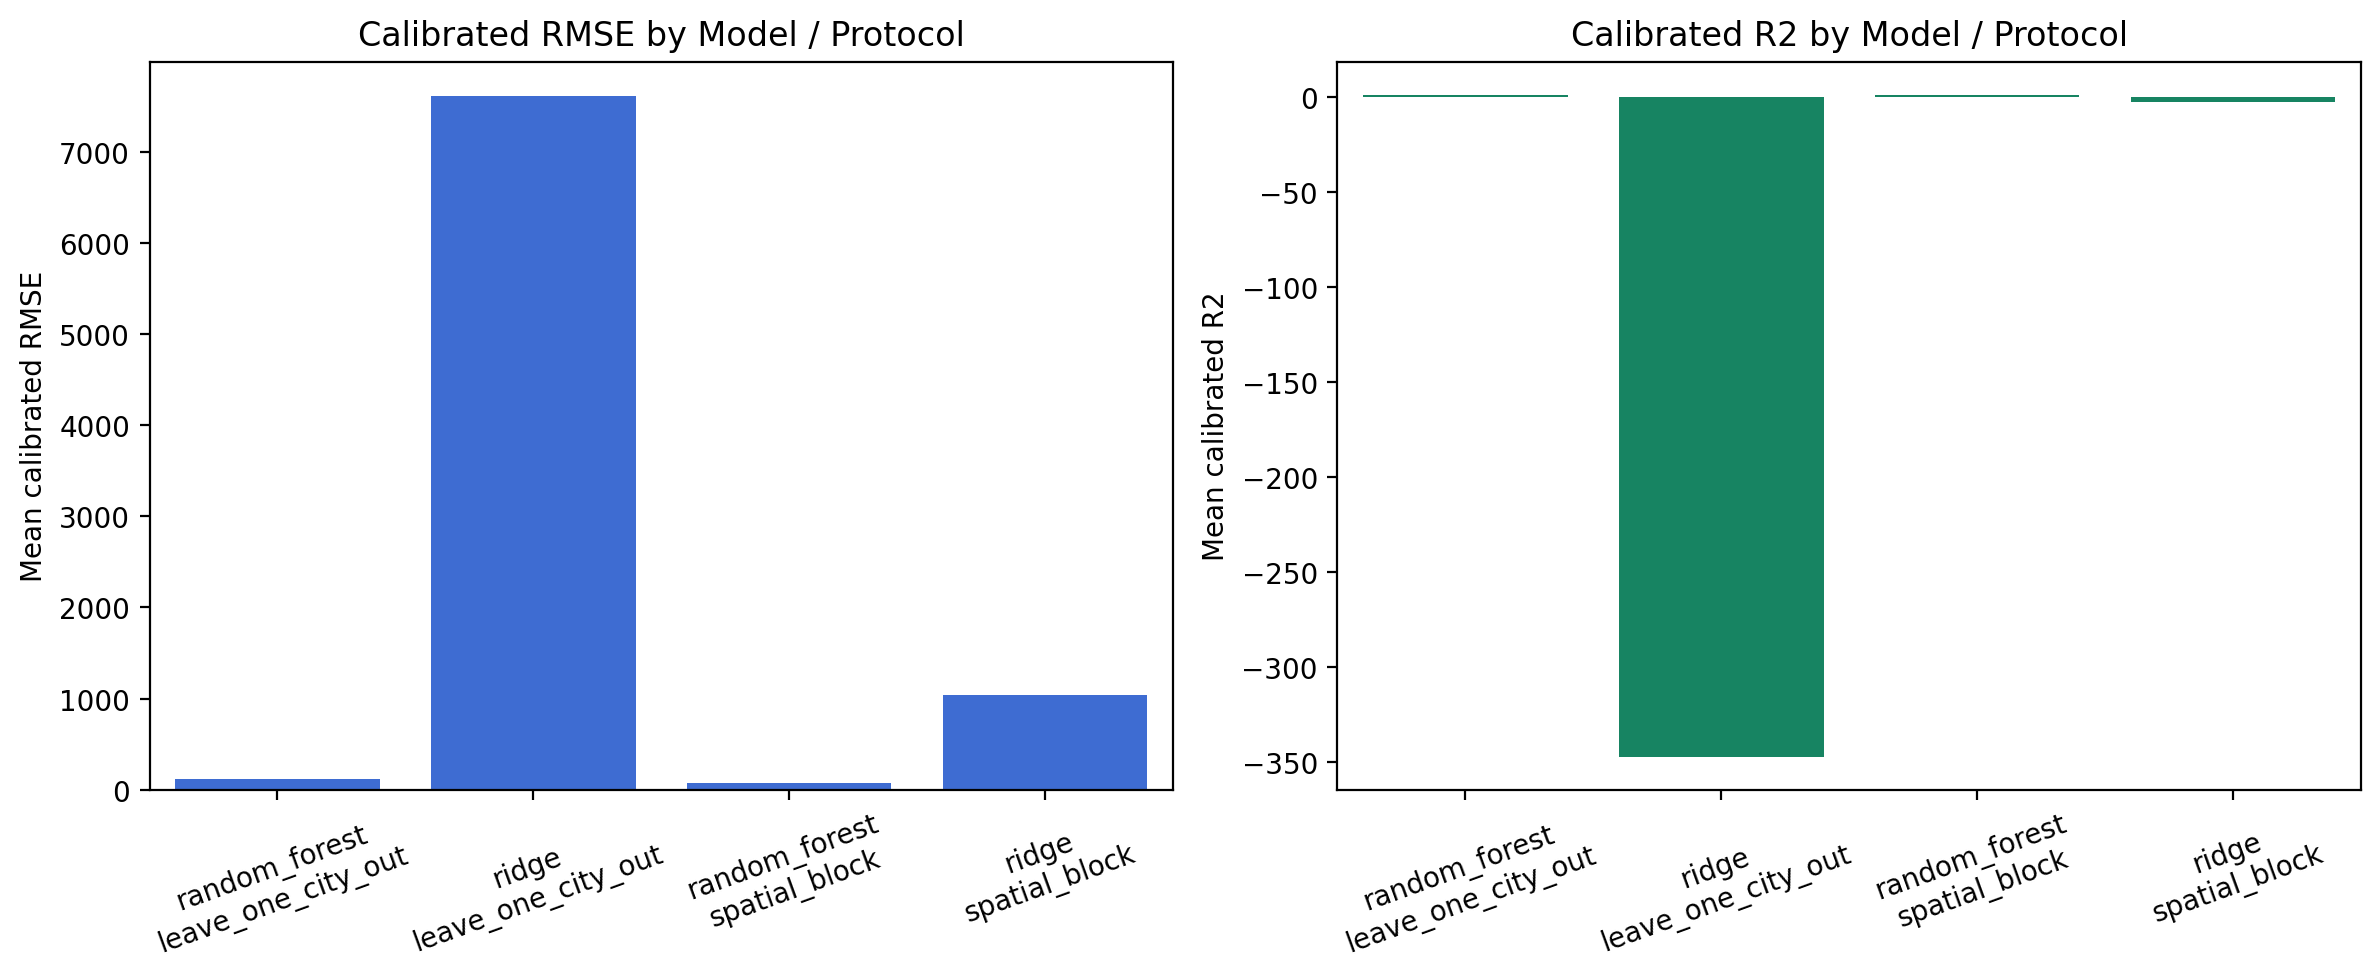
\includegraphics[width=\textwidth]{figures/figure_model_comparison.png}
    \caption{Model comparison}
\end{subfigure}
\hfill
\begin{subfigure}[t]{0.48\textwidth}
    \centering
    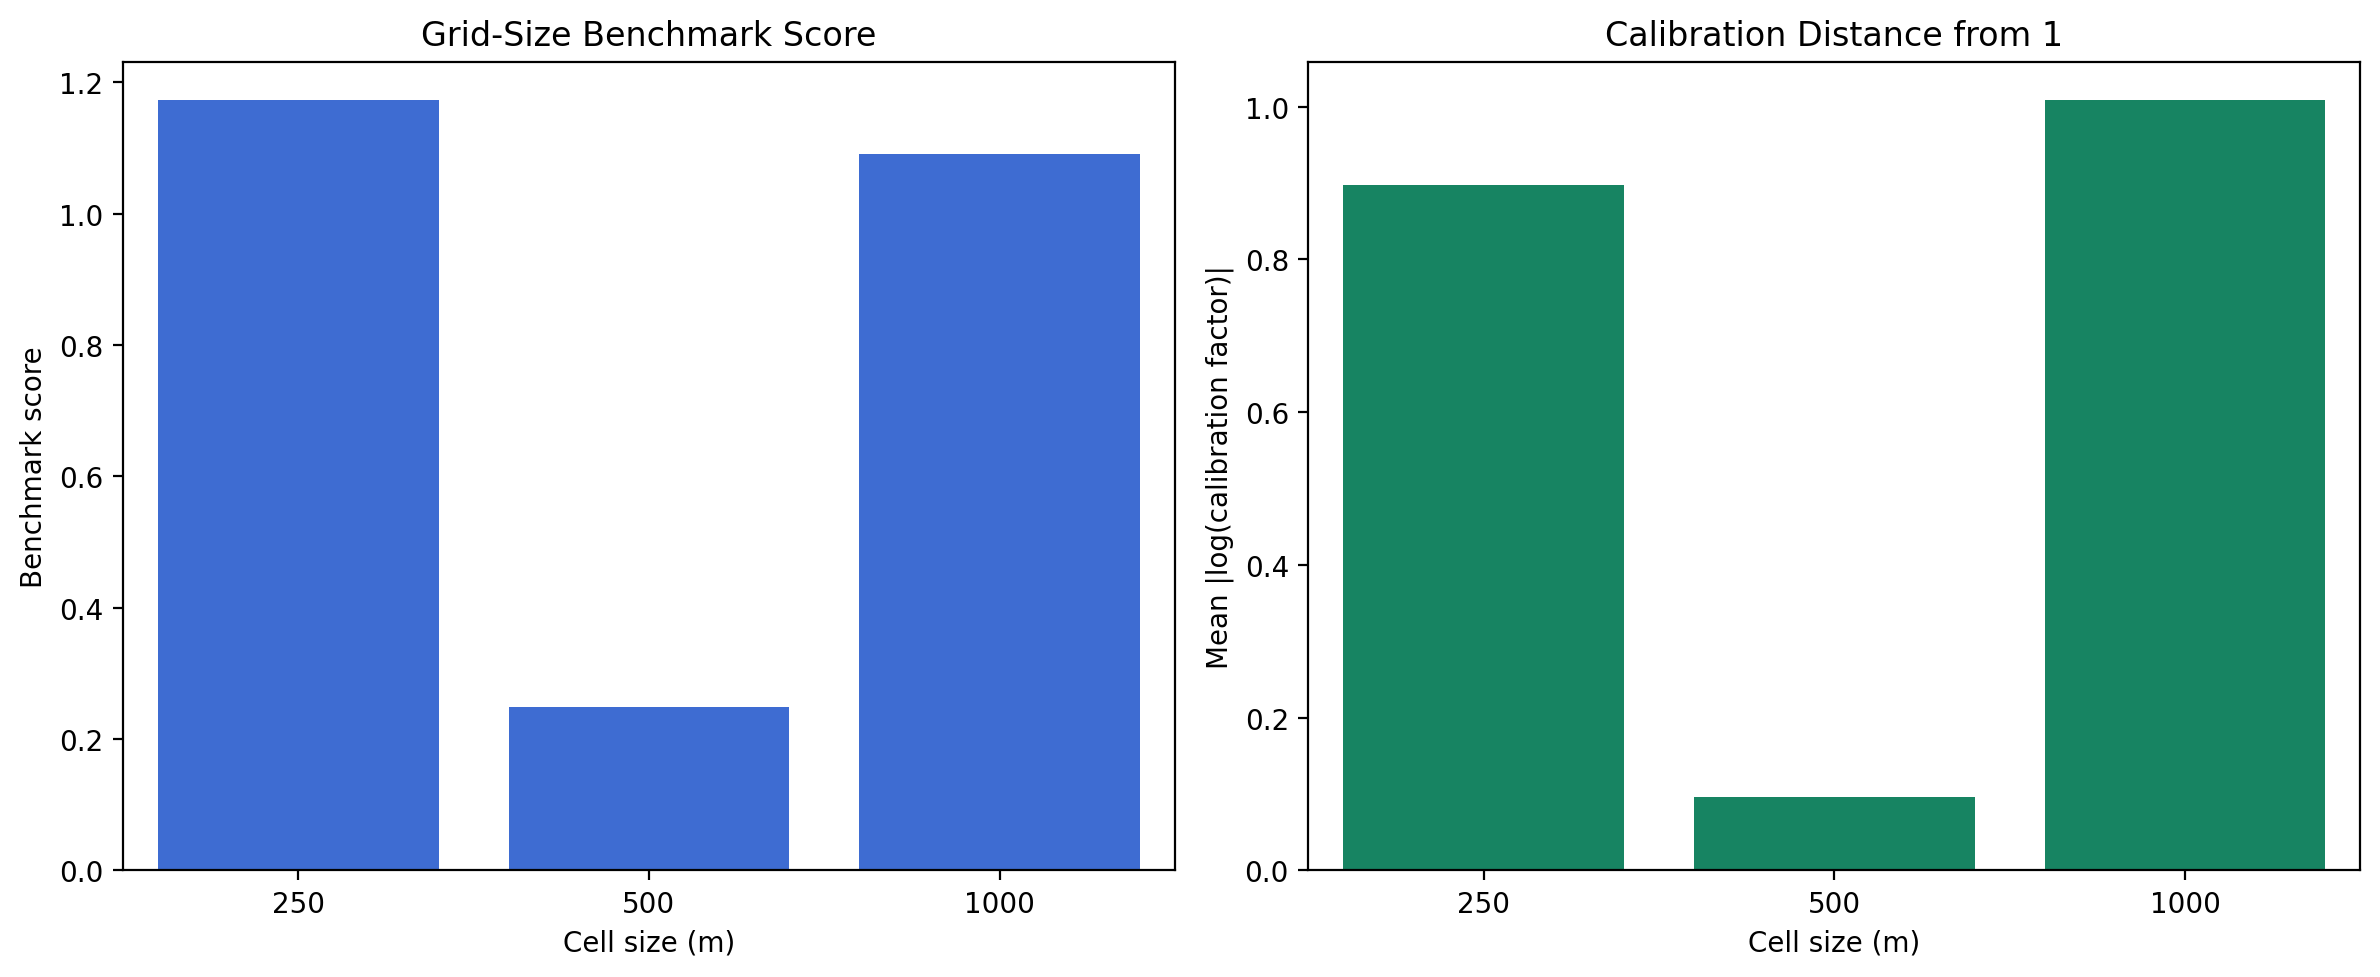
\includegraphics[width=\textwidth]{figures/figure_grid_size_benchmark.png}
    \caption{Grid-size benchmark}
\end{subfigure}
\caption{Quantitative baseline selection for the frozen production configuration. Panel (a) compares candidate models and shows that random forest provides substantially stronger calibrated validation performance than ridge. Panel (b) summarizes the grid-size benchmark and supports 500 m as the default production resolution, balancing spatial detail against stability. Together, the two panels justify the frozen City1 v2 identity: random forest + 500 m + calibrated-only.}
\label{fig:baseline-selection}
\end{figure}

\begin{table}[H]
\centering
\caption{Core model and grid validation summary. The table combines the main model-comparison results with the grid-size benchmark used to lock the frozen 500 m production configuration.}
\label{tab:core-validation}
\begin{tabular}{llllll}
\toprule
Component & Setting & Protocol / grid & Calibrated RMSE & Calibrated $R^2$ & Score \\
\midrule
Model & random forest & LOCO & 115.934 & 0.934 & -- \\
Model & ridge & LOCO & 7609.928 & -347.088 & -- \\
Model & random forest & spatial block & 76.301 & 0.980 & -- \\
Model & ridge & spatial block & 1039.817 & -2.690 & -- \\
\midrule
Grid & frozen default & 500 m & -- & -- & 0.248572 \\
Grid & high detail & 250 m & -- & -- & 1.172821 \\
Grid & coarse & 1000 m & -- & -- & 1.091467 \\
\bottomrule
\end{tabular}
\end{table}


\subsection{District benchmark}

District-level comparison provided uneven but useful internal support. Almaty showed the strongest signal, with Pearson 0.543 and Spearman 0.657. Astana and Shymkent were notably weaker, so this layer should be described as partial internal administrative validation rather than truth validation.

Almaty is the clearest internal support case in the current benchmark package. This is consistent with its stronger OSM completeness context and with the fact that the district comparison there retains at least moderate rank-order agreement after aggregation. By contrast, the weaker or negative correlations in Astana and Shymkent indicate that district-level agreement is heterogeneous across cities and should not be overinterpreted as a solved validation layer. In practice, this means that the district benchmark is informative but bounded: it helps identify where the proxy surface aligns more plausibly with coarse administrative structure, while also making clear that such alignment is not uniform enough to be treated as full intra-urban truth validation.

These weaker district rows should not be read as a collapse of the baseline claim. Rather, they show why a single internal aggregate benchmark is insufficient in this setting. Administrative mismatch, heterogeneous urban form, and differences in open-data support can all weaken agreement once cell-level predictions are aggregated to imperfect district references. The district layer therefore remains valuable precisely because it is partial: it contributes one internal perspective within a broader validation design instead of functioning as the sole arbiter of correctness.

\begin{figure}[H]
\centering
\begin{subfigure}[t]{0.48\textwidth}
    \centering
    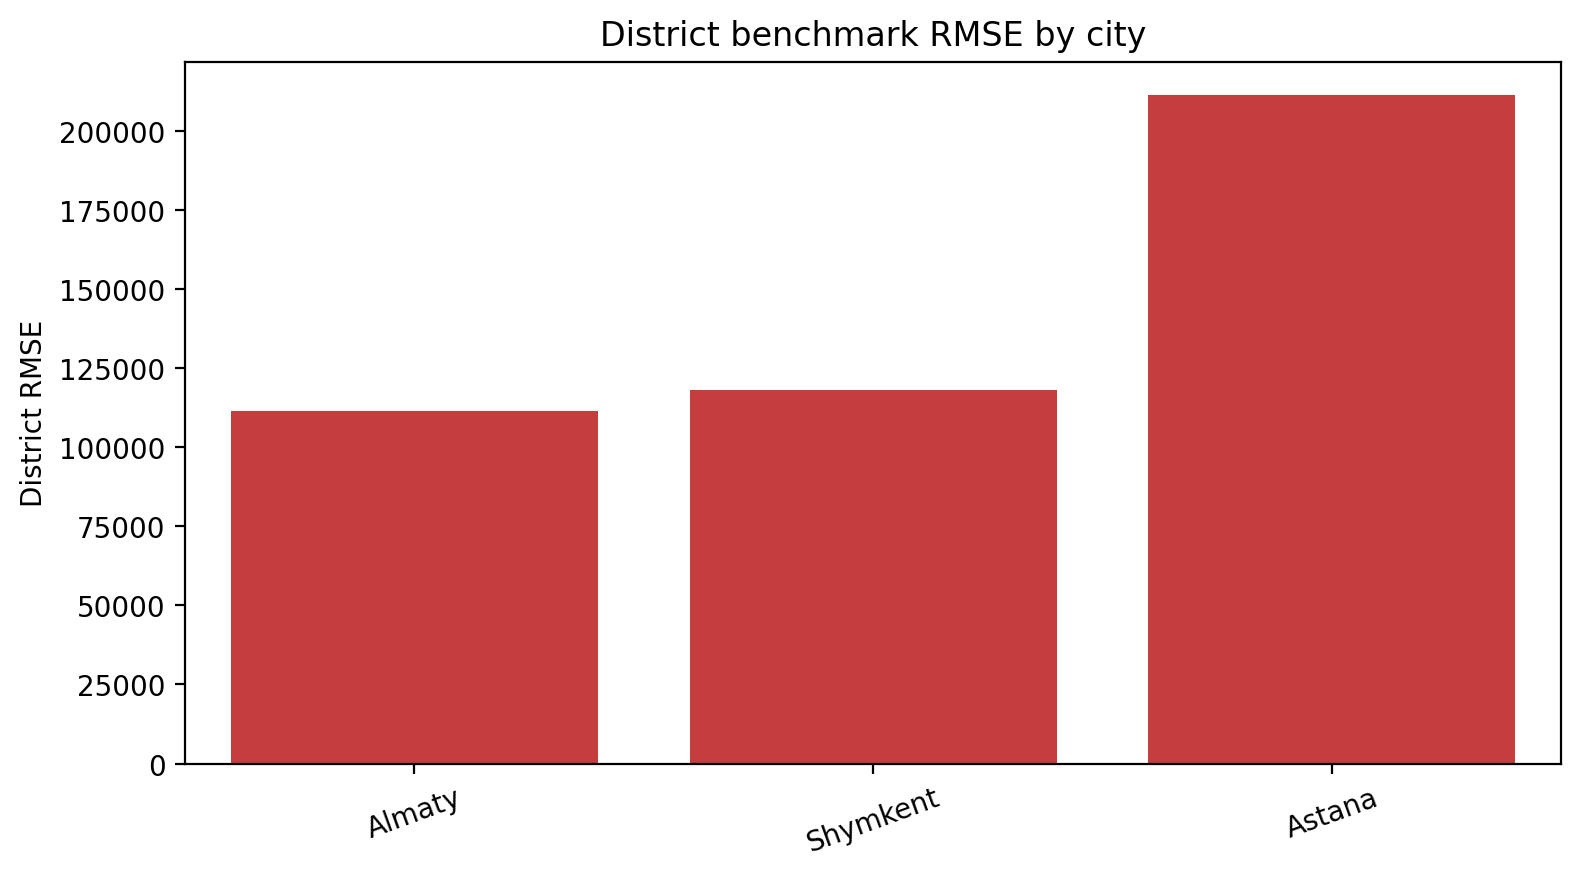
\includegraphics[width=\textwidth]{figures/figure_district_benchmark.png}
    \caption{District benchmark}
\end{subfigure}
\hfill
\begin{subfigure}[t]{0.48\textwidth}
    \centering
    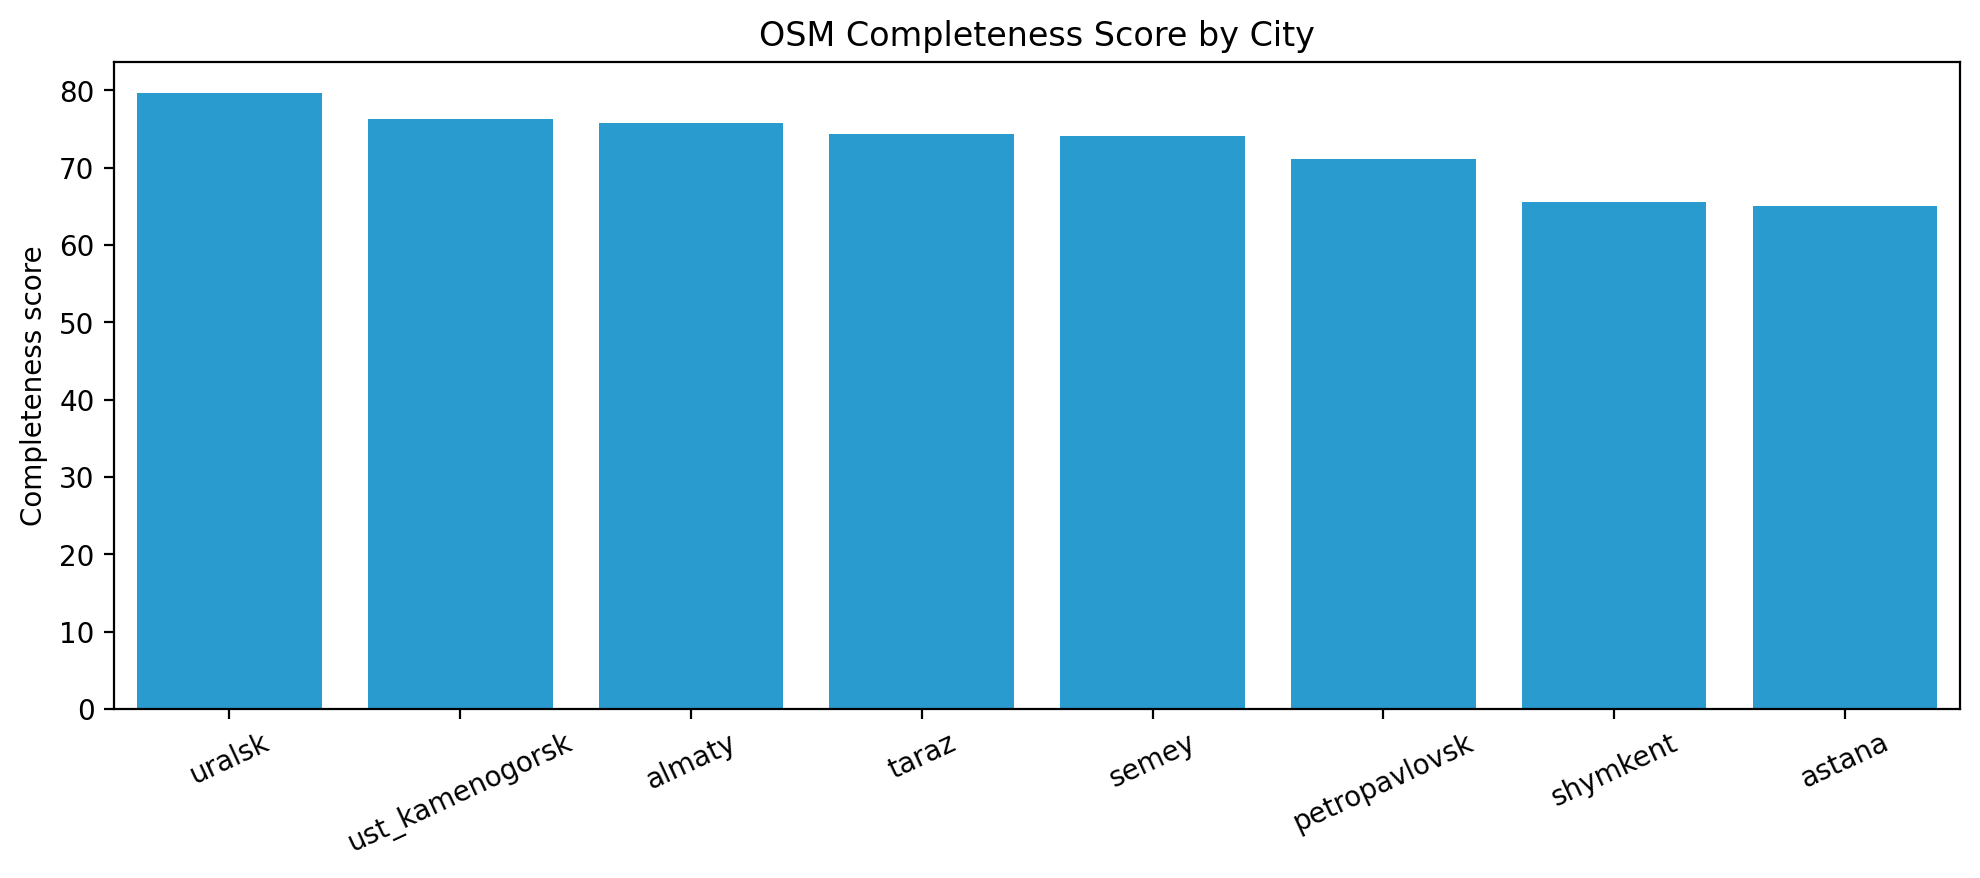
\includegraphics[width=\textwidth]{figures/figure_osm_completeness.png}
    \caption{OSM completeness}
\end{subfigure}
\caption{Internal and input-quality evidence layers. Panel (a) reports district-level comparison across the cities where administrative benchmark data were available; this layer is interpreted as partial internal administrative validation rather than truth validation. Panel (b) reports OSM completeness by city and is used as an input-reliability context for interpreting heterogeneous performance and qualitative confidence, not as a direct measure of model accuracy.}
\label{fig:internal-quality}
\end{figure}

\input{tables_tex/table3_district_benchmark.tex}

\subsection{External benchmark}

External benchmark results supported the structural plausibility of the surface. WorldPop was strongest for overall correlation, reaching Pearson 0.877, whereas GHS-POP was strongest for hotspot-sensitive metrics, with Spearman 0.834, top-decile overlap 0.614, and hotspot IoU 0.443.

This split between WorldPop and GHS-POP is a strength of the evidence stack rather than an inconsistency. WorldPop provides the strongest support for broad agreement in the overall shape of the proxy surface, suggesting that the v2 baseline captures a city-wide spatial structure comparable to an established independent product. GHS-POP, however, aligns more closely with hotspot-sensitive diagnostics, which suggests stronger agreement in the relative placement or concentration of dense urban clusters. Taken together, the two products support complementary aspects of the surface: one at the level of broad structural similarity, the other at the level of dense concentration structure.

The external benchmark should therefore be interpreted as a comparative structural lens rather than as a ranking contest with a single winner. For a baseline framed around proxy population modeling under scarcity, it is scientifically useful that different independent products agree with different parts of the signal. That pattern is more informative than a single undifferentiated comparison score because it clarifies how the surface behaves across multiple notions of similarity without implying that any external product provides cell-level truth.

\begin{figure}[H]
\centering
\begin{subfigure}[t]{0.48\textwidth}
    \centering
    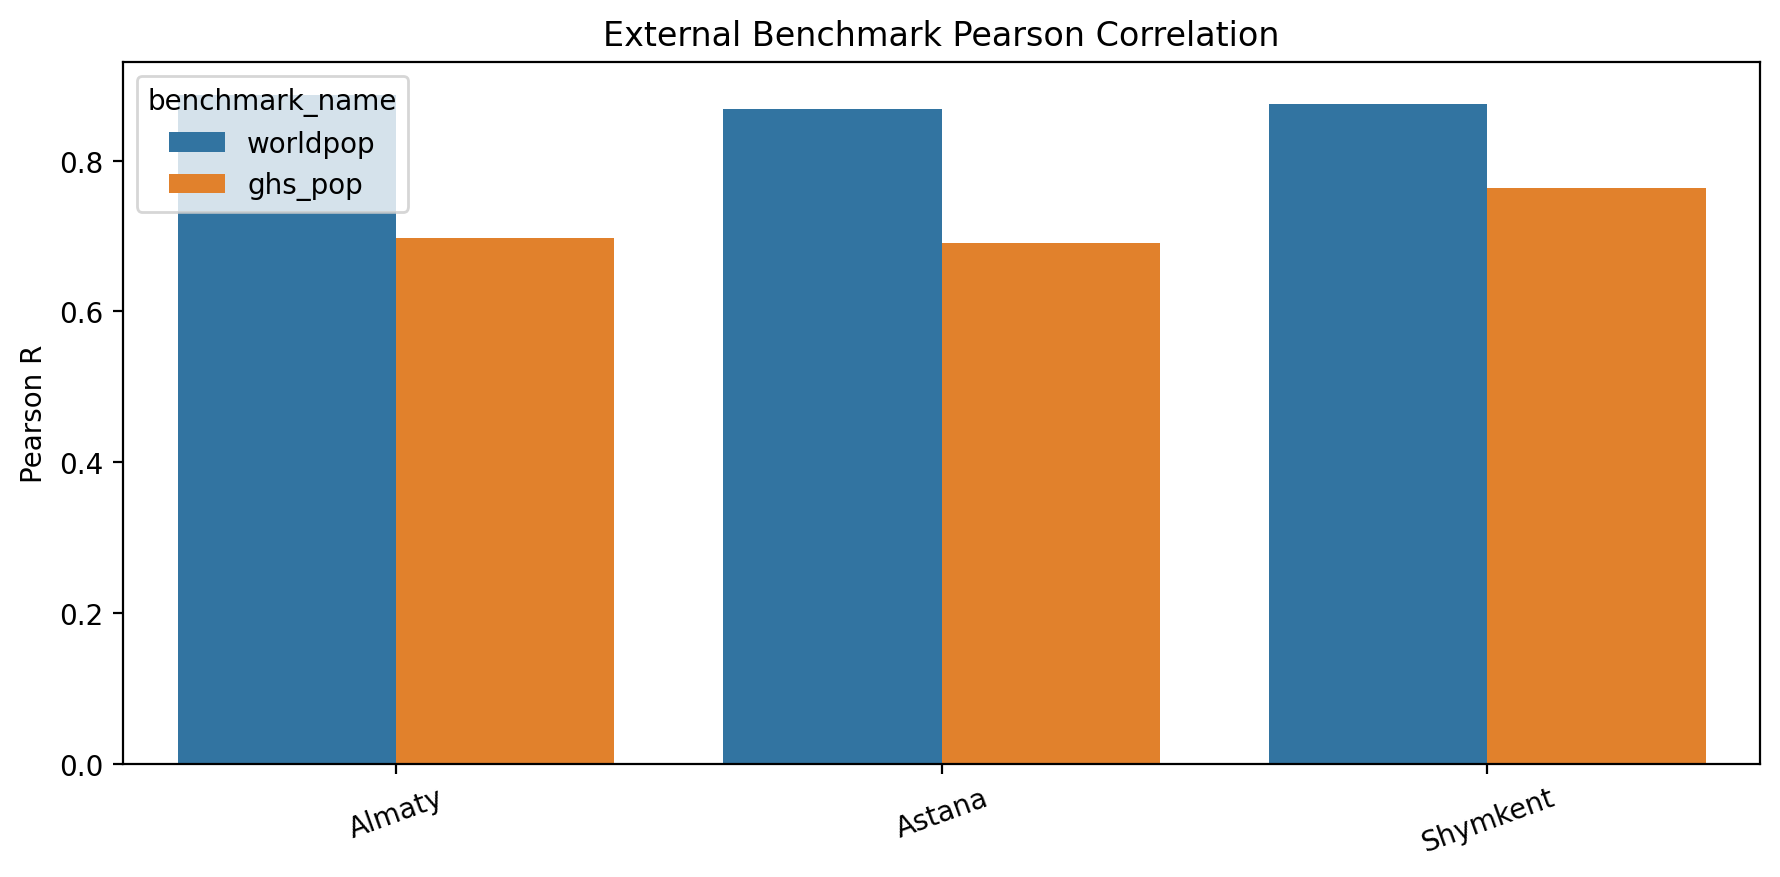
\includegraphics[width=\textwidth]{figures/figure_external_benchmark_pearson.png}
    \caption{Overall correlation}
\end{subfigure}
\hfill
\begin{subfigure}[t]{0.48\textwidth}
    \centering
    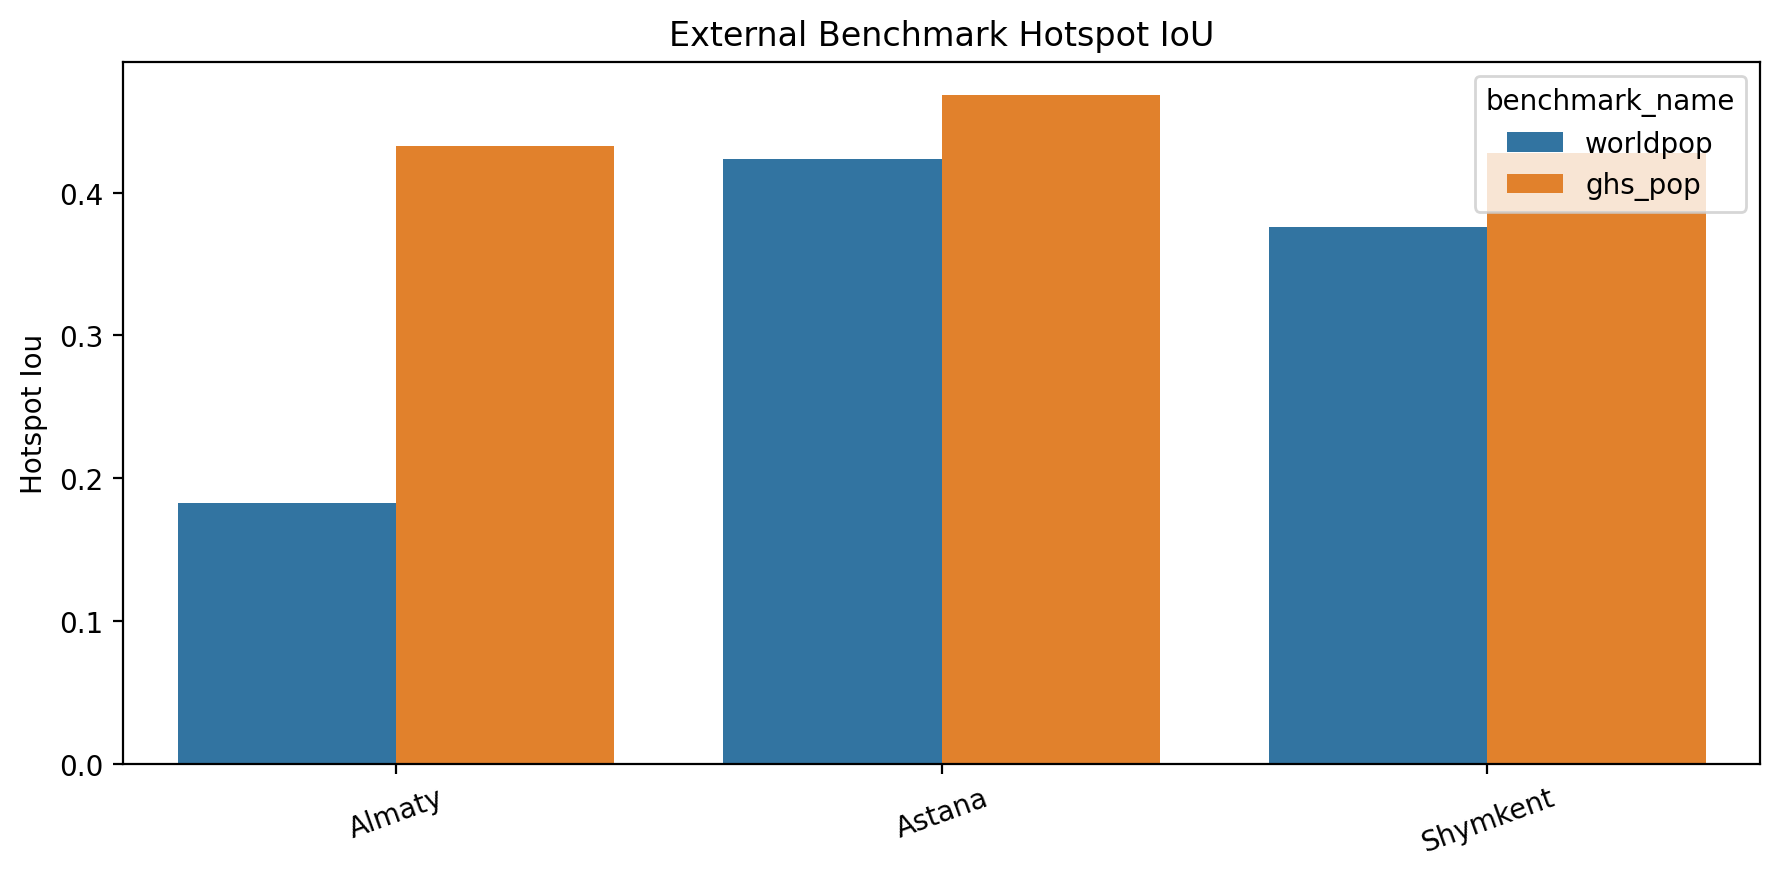
\includegraphics[width=\textwidth]{figures/figure_external_benchmark_hotspot_iou.png}
    \caption{Hotspot agreement}
\end{subfigure}
\caption{External benchmark comparison against independent gridded population products. Panel (a) summarizes overall correlation agreement, where WorldPop provides the strongest support for broad structural similarity. Panel (b) focuses on hotspot-sensitive agreement, where GHS-POP better captures dense concentration structure. The figure is interpreted as external structural comparison rather than validation against ground-truth cell-level census labels.}
\label{fig:external-benchmark}
\end{figure}

\input{tables_tex/table4_external_benchmark.tex}

\subsection{Ablation}

The full frozen feature configuration remained the strongest setting. It achieved a calibrated RMSE of 115.934 and a calibrated $R^2$ of 0.934, while the built-form-only variant was the strongest reduced ablation with a calibrated RMSE of 120.656 and a calibrated $R^2$ of 0.929. The full feature configuration also showed a large calibration RMSE gain of 135.821.

The ablation pattern provides a clear scientific reading of the baseline. Built-form-only is the strongest non-full configuration, which indicates that morphology and built intensity carry the dominant share of the predictive structure in the current proxy setup. At the same time, the full feature stack still performs best overall, showing that transport and service-related variables are not decorative additions: they contribute additional information beyond built form alone, even if their marginal contribution is smaller than that of the built-form core.

The calibration gain is equally important for interpretation. A reduction of 135.821 in RMSE between raw and calibrated full-model outputs indicates that official-total anchoring is a major component of the final product rather than a cosmetic adjustment applied after the fact. In other words, the v2 surface should be understood as the outcome of learned intra-urban differentiation together with explicit city-total consistency. This is central to the paper's baseline identity and helps explain why calibration remains part of the scientific contribution rather than merely a deployment detail.

\begin{figure}[H]
\centering
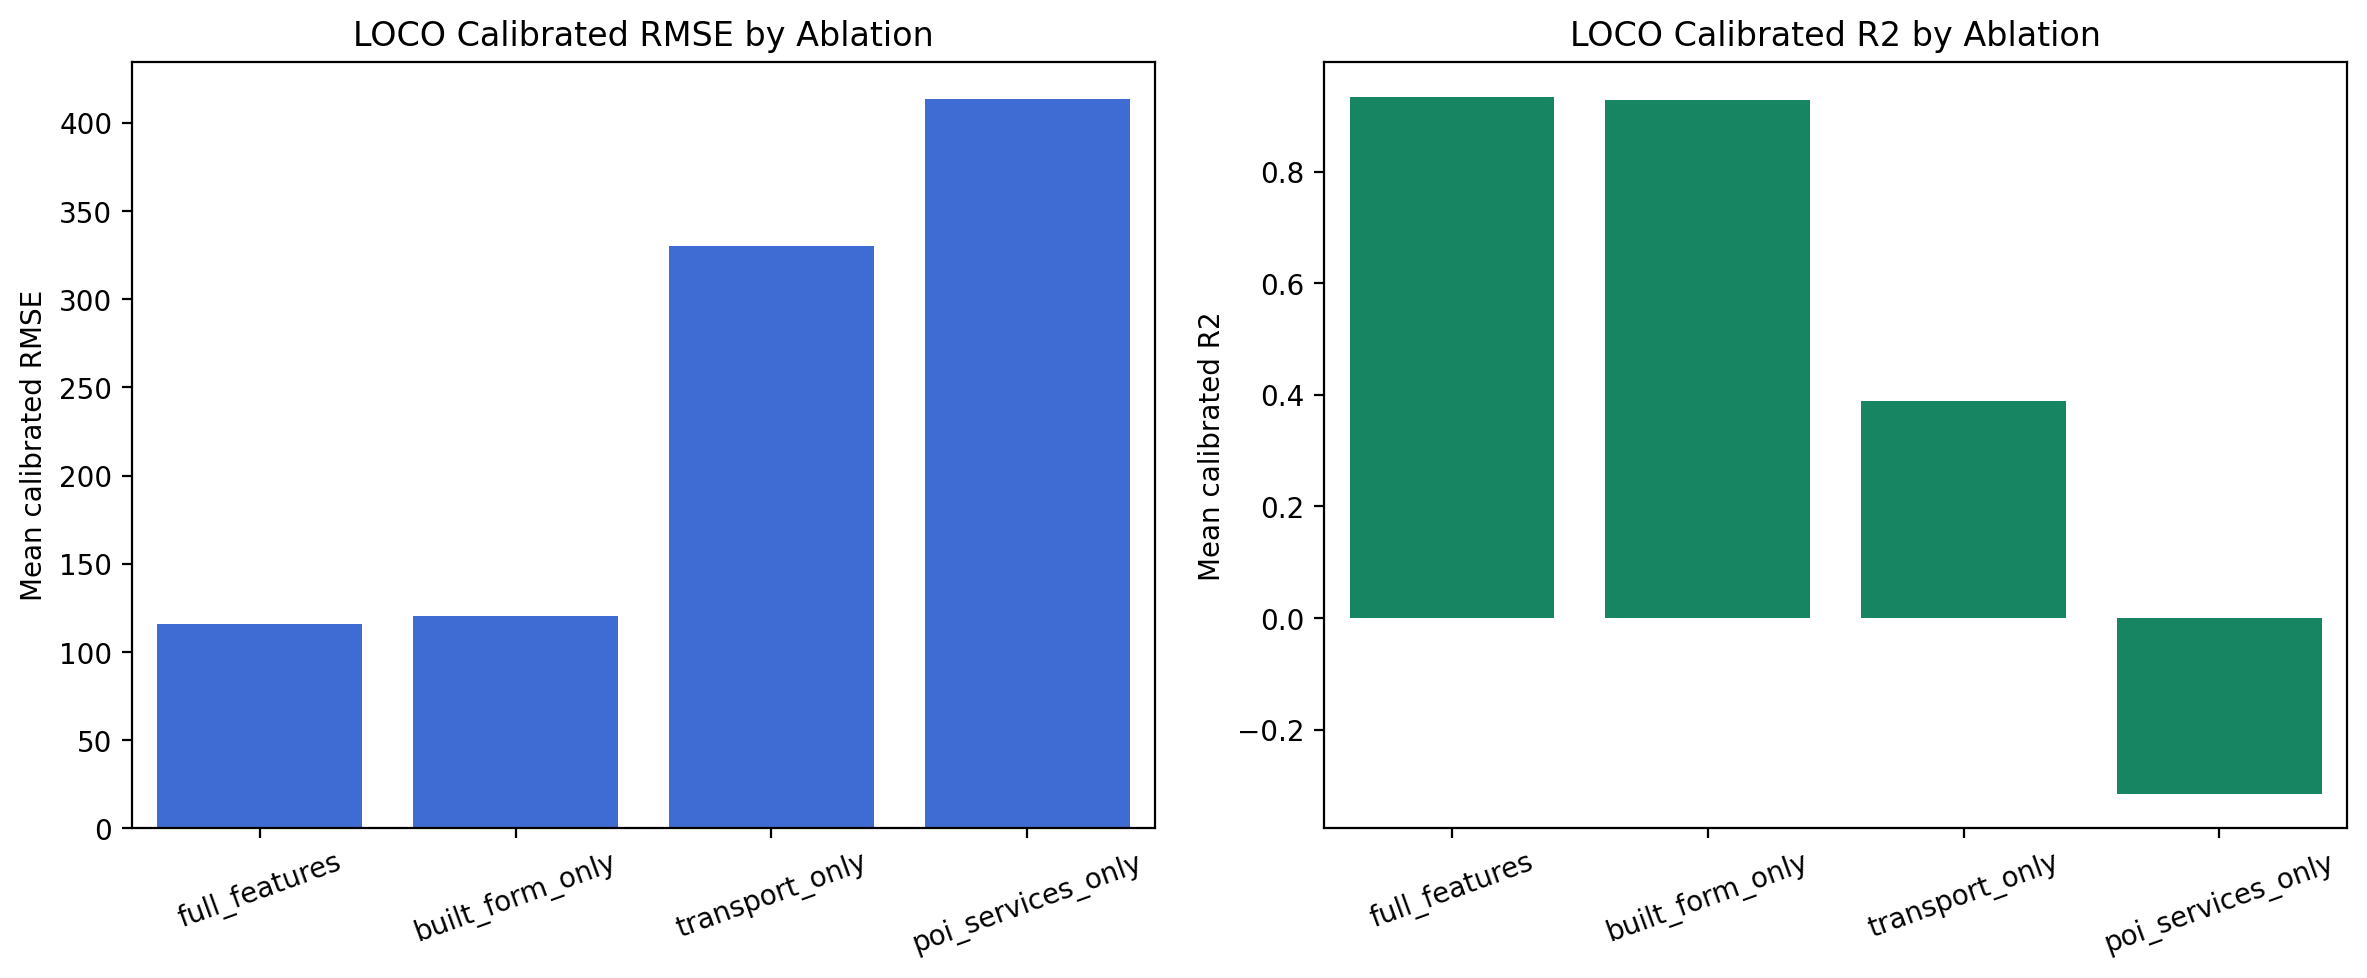
\includegraphics[width=0.78\textwidth]{figures/figure_ablation_loco.png}
\caption{Ablation results under leave-one-city-out validation. The full feature configuration remains the strongest overall, while the built-form-only variant is the strongest reduced ablation, indicating that built-form signals carry the dominant share of predictive structure. The figure also supports the interpretation that calibration materially improves the final proxy surface and should be treated as a core component of the baseline rather than a cosmetic post-processing step.}
\label{fig:ablation}
\end{figure}

\begin{table}[H]
\centering
\small
\caption{Ablation summary under leave-one-city-out validation. The full frozen feature set remains strongest, while the built-form-only variant is the best non-full configuration.}
\label{tab:ablation}
\resizebox{\textwidth}{!}{%
\begin{tabular}{@{}lrrrrr@{}}
\toprule
Ablation & Features & Raw RMSE & Calibrated RMSE & Calibrated $R^2$ & \shortstack{$\Delta$ RMSE\\vs. full} \\
\midrule
Full feature set & 17 & 251.756 & 115.934 & 0.934 & 0.000 \\
Built-form-only & 9 & 258.999 & 120.656 & 0.929 & 4.722 \\
Transport-only & 2 & 379.942 & 330.041 & 0.389 & 214.107 \\
POI/services-only & 5 & 406.750 & 413.785 & -0.315 & 297.851 \\
\bottomrule
\end{tabular}
}
\end{table}


\subsection{Qualitative validation}

Qualitative validation was locked for Almaty and Astana through eight curated cases. Almaty was interpreted in a stronger OSM-completeness context, while Astana required more caution. Across both cities, dense residential and central mixed-use zones tended to receive high predicted population, whereas peripheral open or weak-built zones tended to receive low predicted population.

In Almaty, the qualitative layer is most convincing when read as a consistency check between predicted concentration and visibly dense built structure. The strongest curated hotspot cases coincide with central mixed-use or dense residential fabric, while the principal coldspot cases align with peripheral open or weak-built zones that remain close to zero even after calibration. This pattern supports the interpretation that the baseline is not simply smoothing population mass indiscriminately, but is responding in a spatially plausible way to strong built-environment gradients.

Astana remains more cautious to interpret because its OSM completeness is only moderate, yet the qualitative layer is still useful. The dominant hotspot remains concentrated in the city's structured central core, while low-intensity gaps remain plausible where built-form signals are weak. This does not eliminate ambiguity, but it does show that the final surface preserves an interpretable urban morphology even in a more weakly supported mapping context. Detailed hotspot and coldspot panels are retained in the supplement so that the main paper can keep the city-level overview while still providing case-level plausibility evidence for readers who want closer inspection.

\begin{figure}[H]
\centering
\begin{subfigure}[t]{0.49\textwidth}
    \centering
    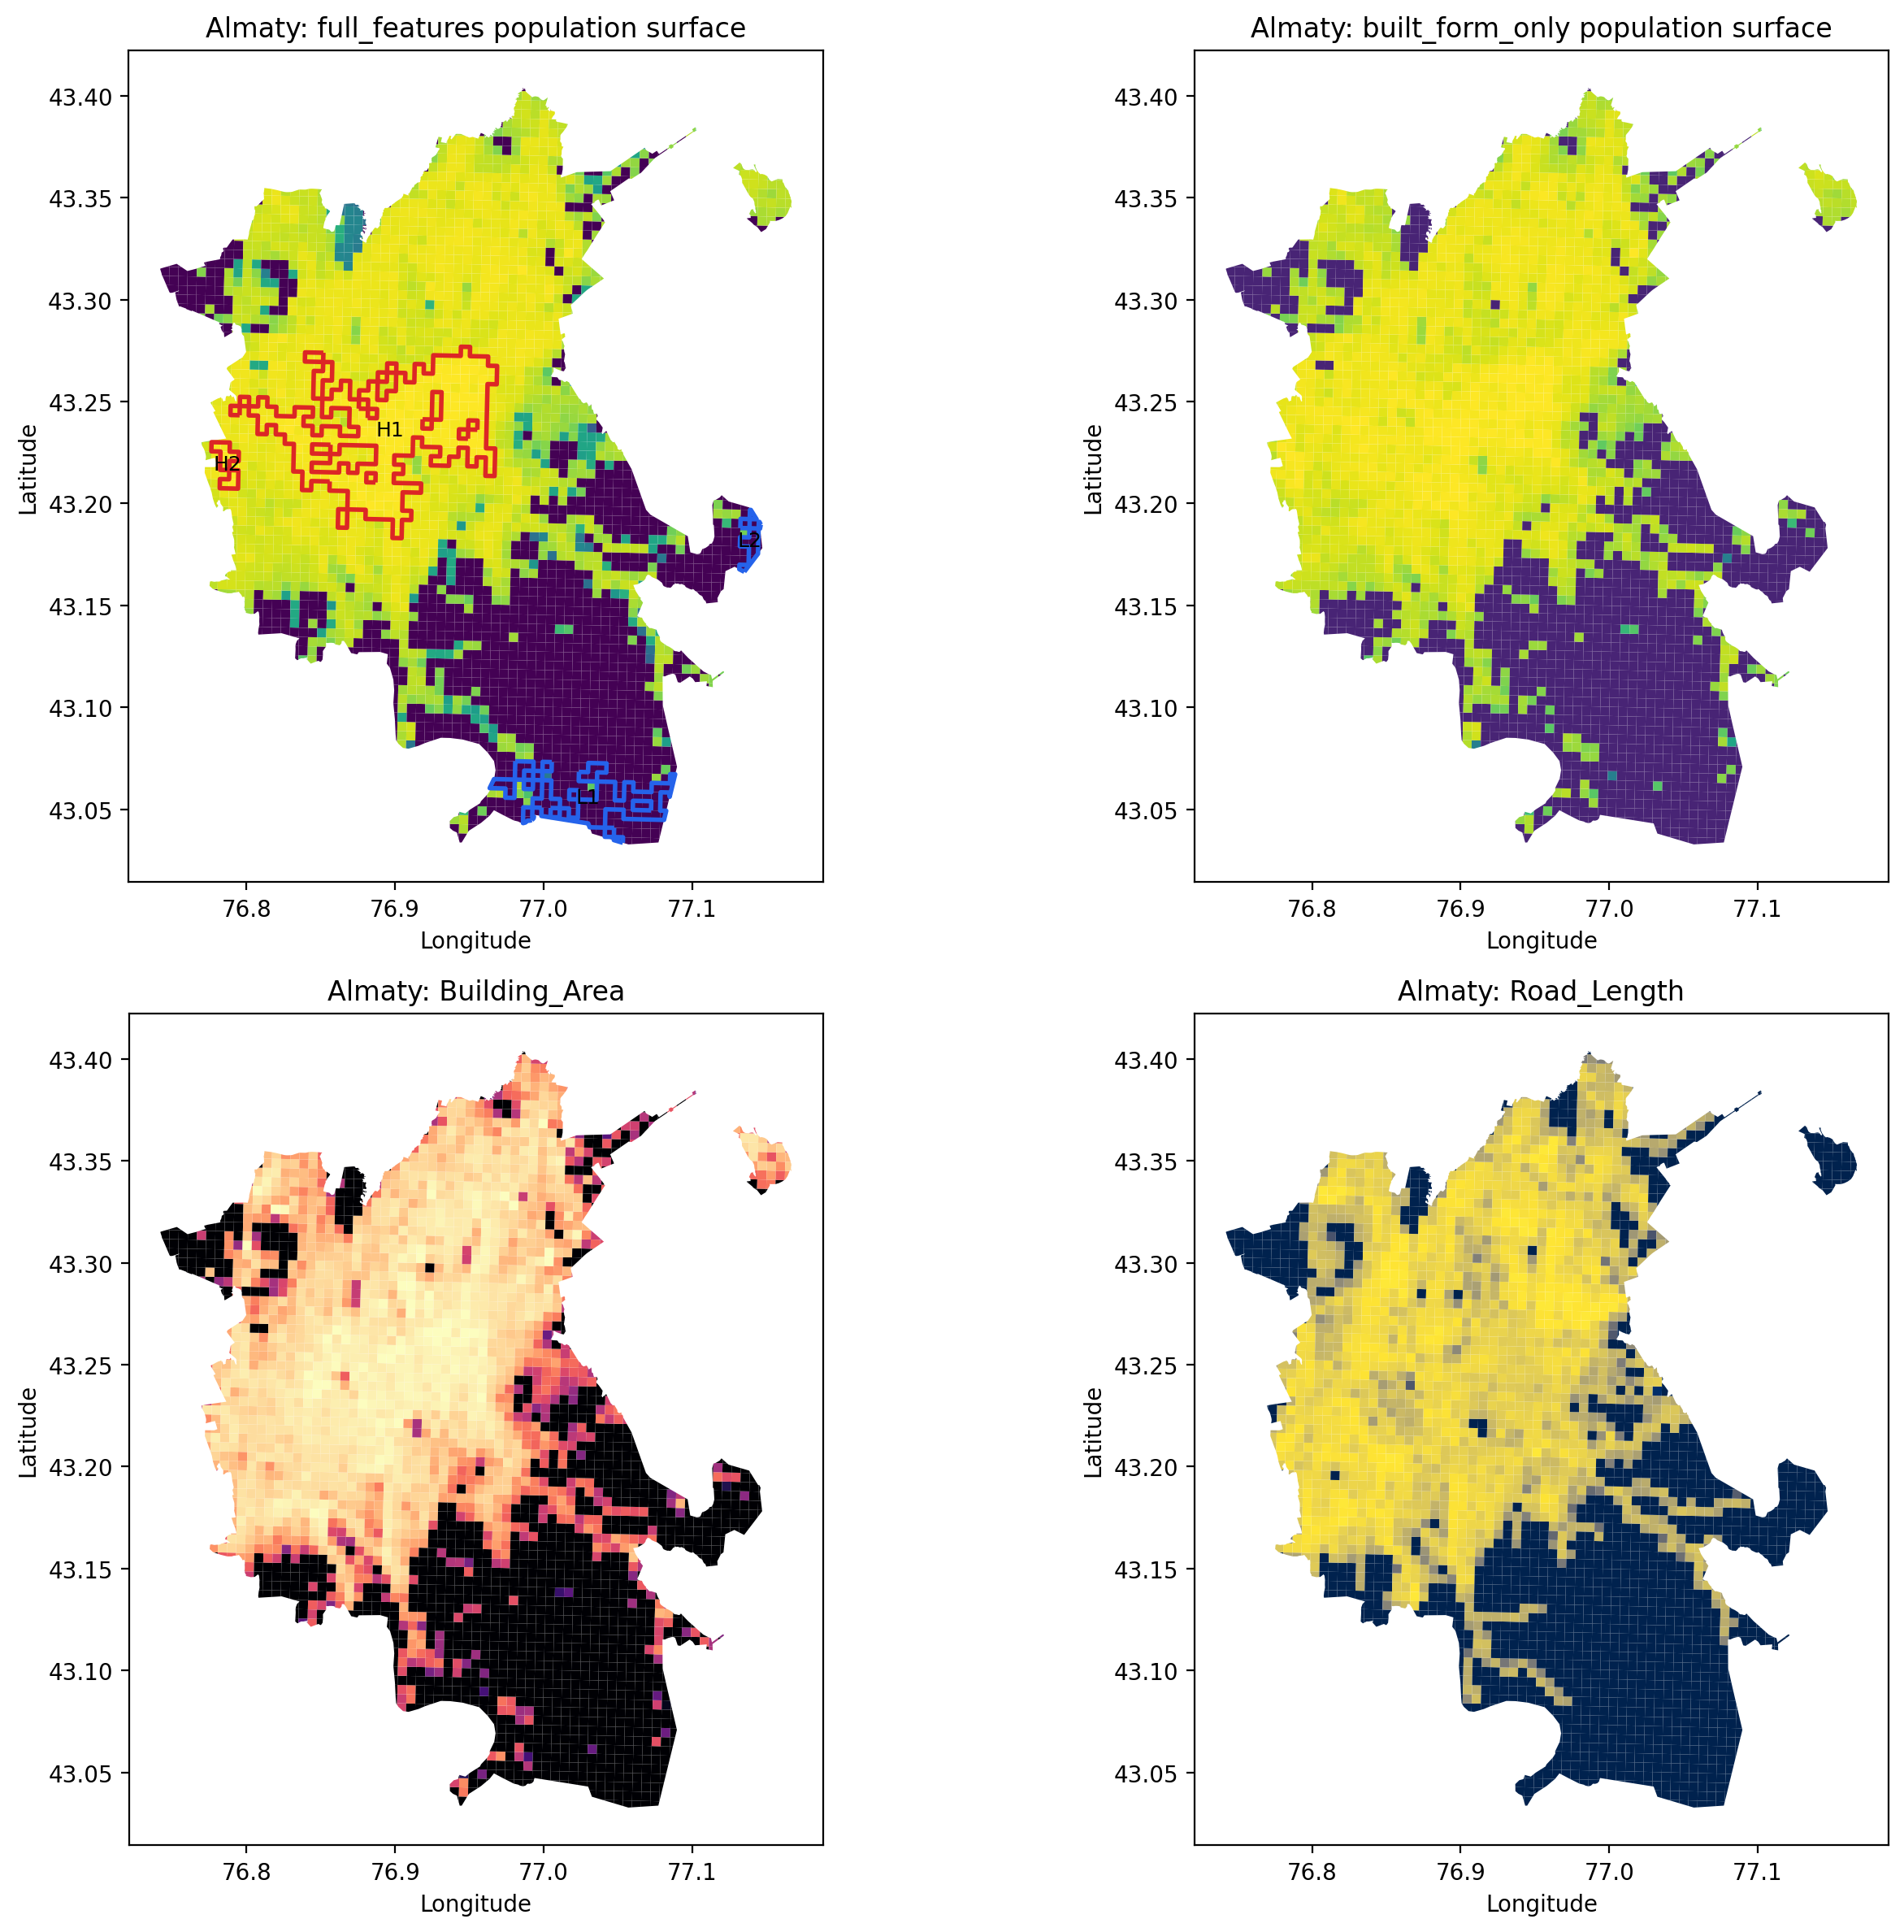
\includegraphics[width=\textwidth]{figures/figure_qualitative_overview_almaty.png}
    \caption{Almaty overview}
\end{subfigure}
\hfill
\begin{subfigure}[t]{0.49\textwidth}
    \centering
    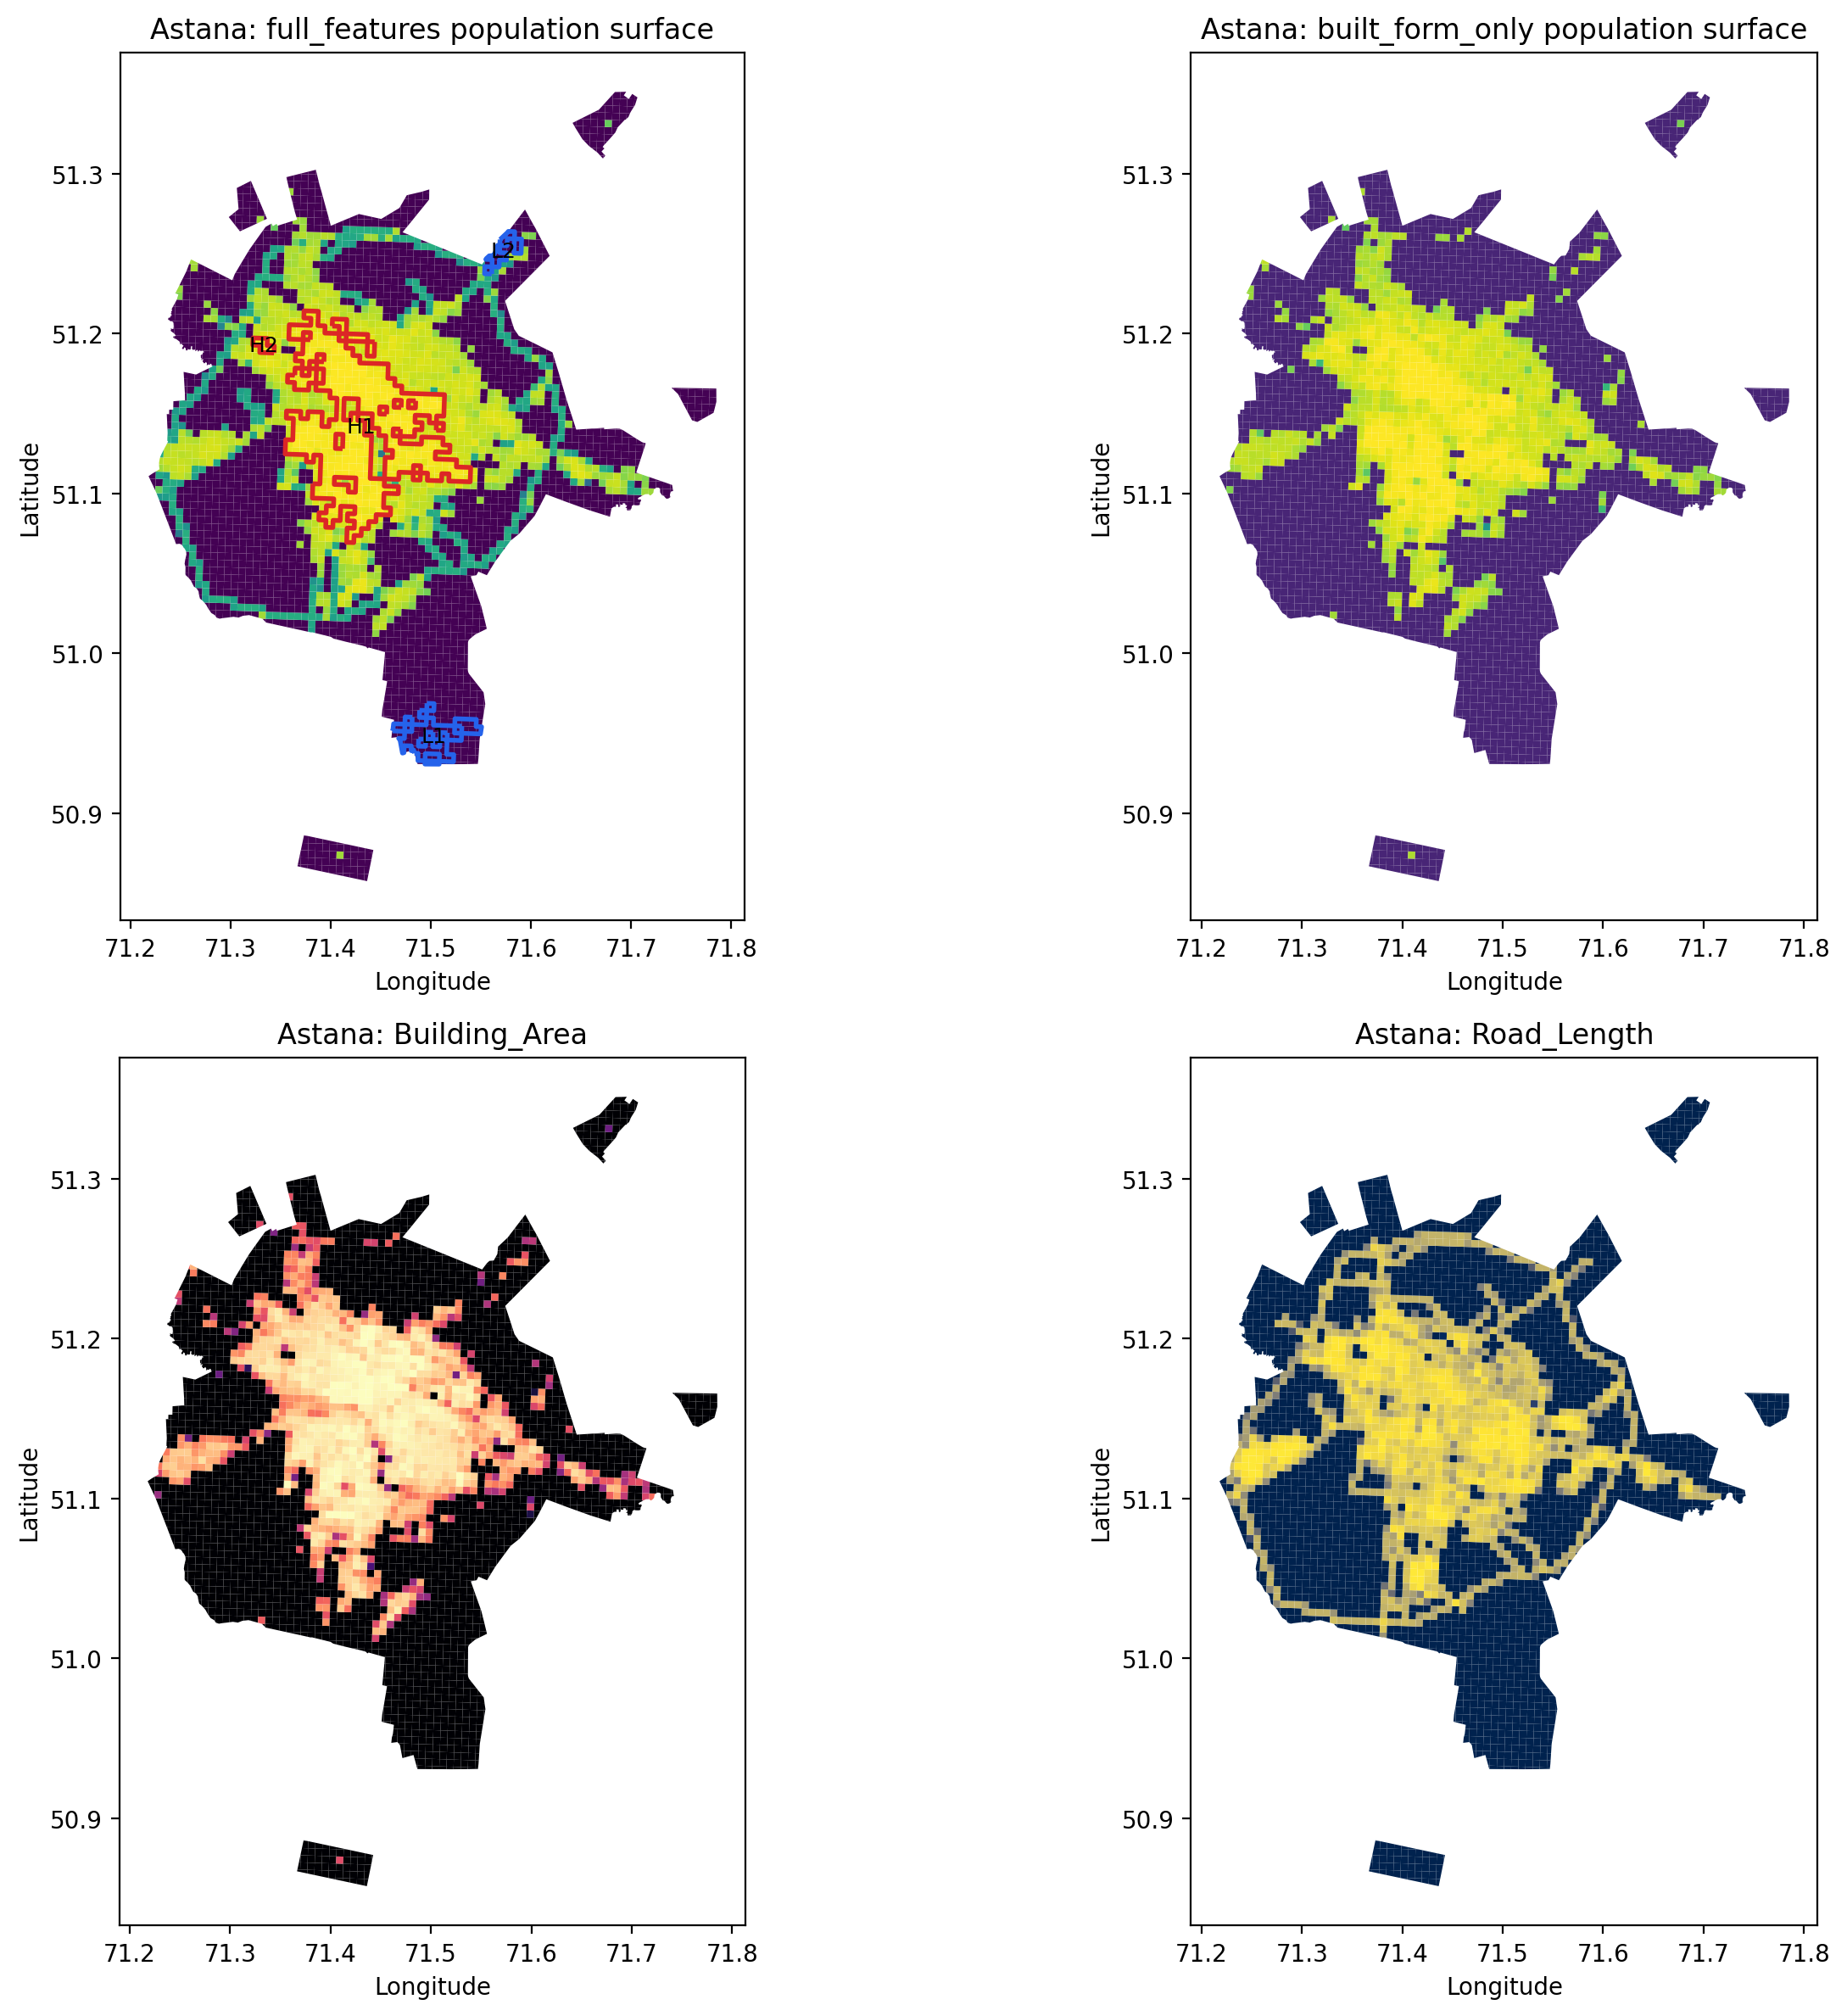
\includegraphics[width=\textwidth]{figures/figure_qualitative_overview_astana.png}
    \caption{Astana overview}
\end{subfigure}
\caption{Qualitative validation overview for the two curated cities, Almaty and Astana. The overview maps compare the final proxy population surface with supporting built-environment layers to assess whether dense residential and central mixed-use areas receive higher predicted population while peripheral open or weak-built zones remain comparatively low. These maps are presented as plausibility evidence and urban-structural interpretation, not as cell-level truth validation.}
\label{fig:qualitative-overview}
\end{figure}

\subsection{Interpretation and Practical Implications}

Taken together, the results support a reading of City1 v2 as a useful analytical baseline rather than as a truth-recovery model. The strongest evidence does not come from any single metric in isolation, but from the convergence of transfer validation, within-city robustness checks, external structural comparison, ablation, and qualitative plausibility. This matters for applied use. In data-scarce urban settings, analysts often need a city-consistent surface that is explicit about what it knows and what it does not know. The frozen v2 package supports that use case by pairing official-total calibration with a bounded but transparent account of where the surface is structurally plausible.

This framing also clarifies how to interpret heterogeneous evidence. The weaker district rows for Astana and Shymkent do not erase the broader baseline claim; instead, they mark where administrative aggregation remains a partial and imperfect lens. Likewise, the split between WorldPop and GHS-POP is not a contradiction to be resolved by declaring a single winner. It indicates that different independent products support different aspects of the inferred surface, with one aligning more closely to broad rank-order structure and the other to dense hotspot concentration. For a paper explicitly framed around missing cell-level truth, that complementarity is more useful than a false impression of a single definitive benchmark.

Within those bounds, the baseline is already practically useful for exploratory intra-urban comparison, service-planning screening, hotspot-aware triage, and city-level prioritization in data-scarce contexts. It can inform questions such as where dense concentration is most plausibly located, where coarse administrative support is stronger or weaker, and where open-data completeness warrants more or less interpretive confidence. At the same time, the surface should not be used as if it were an exact cell-level census product or as a substitute for truth-validated accounting below the support actually available in the current evidence stack. The value of City1 v2 lies in making those boundaries explicit while still offering a reproducible and empirically supported analytical surface.

Detailed curated hotspot and coldspot panels for Almaty and Astana are retained as supplement material rather than placed in the main paper, since they serve primarily as supporting plausibility evidence after the city-level overview maps.
